\section{Thread}


\subsection{Introduction}
Nowadays, the term "Smart Home" is more and more often used in the media or on the internet. According to a survey by \href{https://www.statista.com/outlook/dmo/smart-home/worldwide#smart-homes}{statista.com}\cite{Statista}, the share of the global market for smart homes will reach US\$100 million by the end of 2021 and double that number by 2025. The aim of smart homes is to enable the owner or occupant of the home to easily control the devices in their home via a smartphone or over the internet. Such devices could include smart thermostats, light switches and power sockets. The examples listed above are just a small selection of the wide range of these devices, as there are countless other consumer electronics, security or control electronics (such as irrigation systems) on the market. On the other hand, it is also very important to minimise energy consumption, as environmental protection is becoming increasingly important in society and it is not always possible to supply a thermostat with continuous mains voltage. The \href{https://www.threadgroup.org/}{Thread}\cite{threadgroupurl} provides a solution to this market and these problems.
It is also safe, as the possibility of connection is limited to a given device (this process will be discussed in detail in a later section) and communication is only between devices on the same network. The network topology is considered reliable as several devices are connected to several devices (mesh networking), so that if one device fails, the entire subnetwork does not collapse. This is also due to the fact that devices dynamically choose their role in the network. Low-power Thread devices can run for years on a single lithium coin-cell battery. Last but not least, thousands of devices can be connected to a Thread network, providing a potential solution for connecting devices in smart offices.

\subsection{Thread comparison with other protocols}
First of all, this thesis discusses the differences between well known mesh protocols, like ZigBee and Bluetooth Mesh and compares the differences between them. Finally the Wi-Fi is also compared, which is the most widely used wireless radio protocol in the whole world.\cite{threadcompare}\cite{threadcomapare2}

\subsubsection{Thread vs. ZigBee}
ZigBee is the closest data link protocol to Thread. It's physical layer and the \textit{Medium Access Control} (short \textbf{MAC}) layer in the data link layer are defined by the same standard as IEEE 802.15.4. The modulation type is \textit{Carrier sense multiple access/collision avoidance} (short \textbf{CSMA/CA}), which ensures good, secure data transmission on unused channels. Thus, both communications have a data rate of 250\,\si{\kilo bit/s}, making the use of this technology for smart home solutions a highly reliable and low latency solution. This standard defines three different frequencies as carrier frequencies, but the most relevant one used in my bachelor's thesis is 2.4\,\si{\giga\hertz}, because both protocols are based on it. This range falls in the ISM (Industrial, Scientific, Medical)  band in all countries and therefore does not require a licence. Thread protocol was specified in 2016 and has significant innovations compared to ZigBee which has been in development since 2003. Thread is a self-healing mesh network based on IPv6 (as opposed to Zigbee, which is based on IPv4) and is designed for low-power IoT device communication. Unlike IPv4 addressing, which uses a 32-bit number (4.3 billion distinct addresses can be reserved), IPv6 uses 128-bit numbers for addressing, giving $3.4 \cdot 10^{38}$ distinct addresses for devices and dedicated IP addresses. This method allows each device to have an unique address, thus facilitating the role of the router in the Internet world. On the other hand the devices determine their own roles in the Thread network dynamically. Both protocols (Thread and ZigBee) fully map the network and determine the endpoint for each packet. For both, a single coin-cell battery is sufficient to power the device up to few years.

\subsubsection{Thread vs. Bluetooth Mesh}
Bluetooth Mesh offers a solution for the automation of industrial buildings and smart homes. Unlike the former, it is based on the IEEE 802.15.1 standard and within it \textit{Bluetooth Low Energy} (short \textbf{BLE}). The advantage of this protocol is that all layers involved in the network model are controlled by the Bluetooth Special Interest Group. BLE also uses the 2.4\,\si{\giga\hertz} carrier frequency with GFSK (Gaussian frequency-shift keyring) modulation. Unlike Thread, Bluetooth Mesh uses flooding to send information to endpoints, which has the disadvantage that it can hold up packets, increasing the latency of a packet. One of its advantages over Thread is that it can send up to four times more data per second. Like Thread and ZigBee, devices with this BLE protocol also can be powered with a coin-cell battery.

\subsubsection{Thread vs. Wi-Fi}
Wi-Fi technology has been around since 1997 and is the most widely used protocol for wireless data transmission. The currently most widely used Wi-Fi 5 (802.11ac) can reach 3.5\,\si{\giga bit/s}, that is 14000 times faster than Thread. However, this speed comes at a cost, as the transceiver module can draw much more power, so powering it from a single coin-cell battery is an impossible task and it requires constant power source (e.g. from power line). Basically the Wi-Fi system has a star point network topology, where a router is the central element of the network, where the devices can be connected, but mesh networking is also supported in the latest Wi-Fi 6. It is commonly referred to as the best speed vs. energy efficient communication method, but it is unsuitable for small and extra low power devices. 


\subsection{Latency comparison between Thread, ZigBee and Bluetooth Mesh}
Silicon Labs conducted a larger scale measurement with their own devices to compare the difference between the latencies of Thread, ZigBee, Bluetooth Mesh. Furthermore, they also made a measurement of the distribution of latencies. These three solutions target the same low-power IoT device market. This measurement was carried out in a large office building. I present two measurement cases in this thesis section.

\subsubsection{First measurement}
\begin{figure}[!htb]
    \centering
    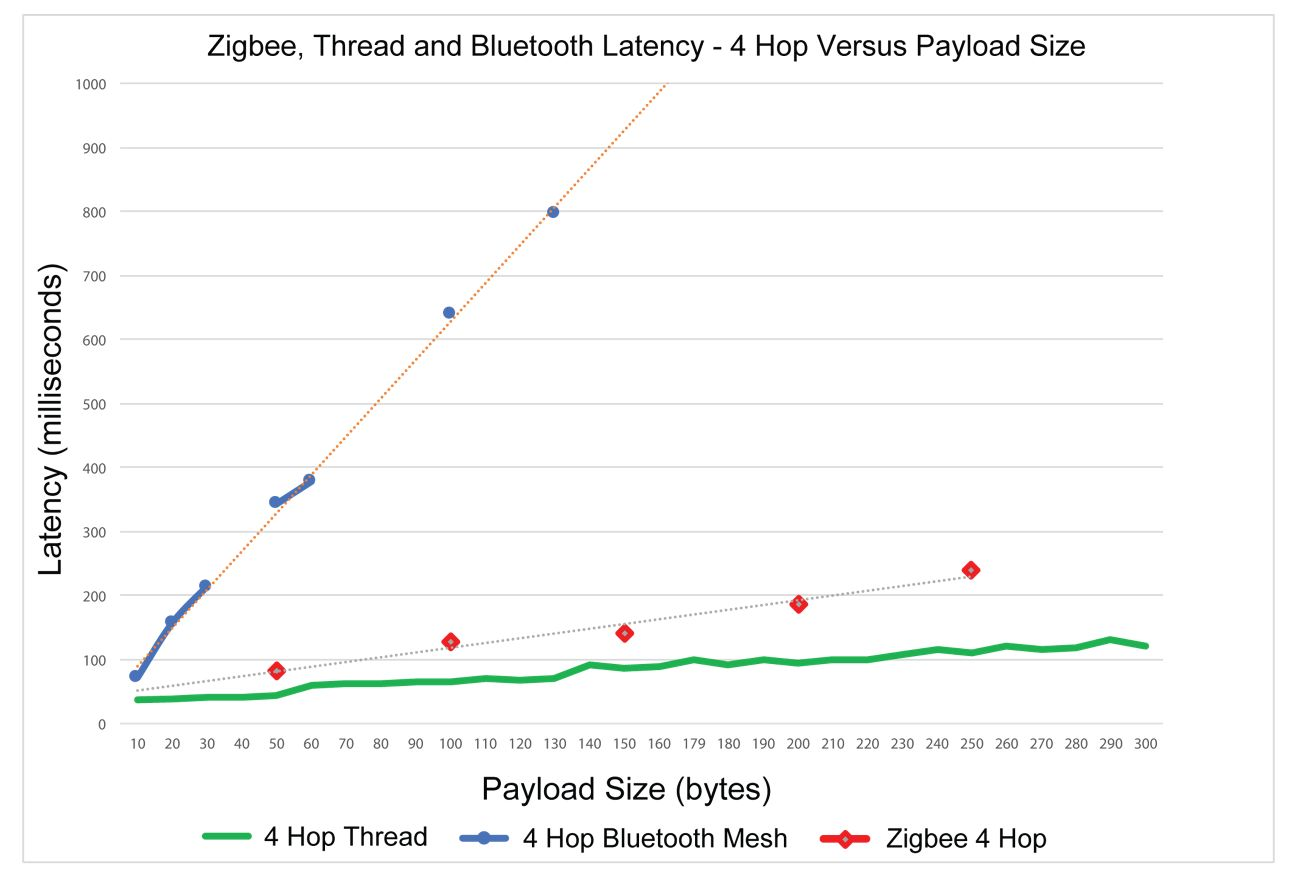
\includegraphics[width=\textwidth]{img/mesh-latency-over-four-hops.png}
    \caption{Mesh network latency between four devices}
    \label{fig:threadoverfourhops}
    \cite{threadSilabs}
\end{figure}
\noindent
The first measurement shows how the latency depends on a given data packet size across four devices. This measurement is presented in Figure \ref{fig:threadoverfourhops}, which shows the latency for very small data (10 bytes). In all three cases there is only very little difference in latency. As the size of the data increases, the latency increases in all cases in different degrees. The measurement results show that as the data packet size increases for Bluetooth Mesh (blue dots), the latency also increases dramatically compared to Thread (green line) and ZigBee (red dots). ZigBee produces much better results than Bluetooth Mesh, but Thread has the smallest slope of the approximate line. However, this measurement only tests the latency dependence between four devices, which is not the intended use of mesh networks, as the point of a mesh network is to have many small devices, up to thousands, connected to each other.


\subsubsection{Second measurement}
\begin{figure}[!h]
    \centering
    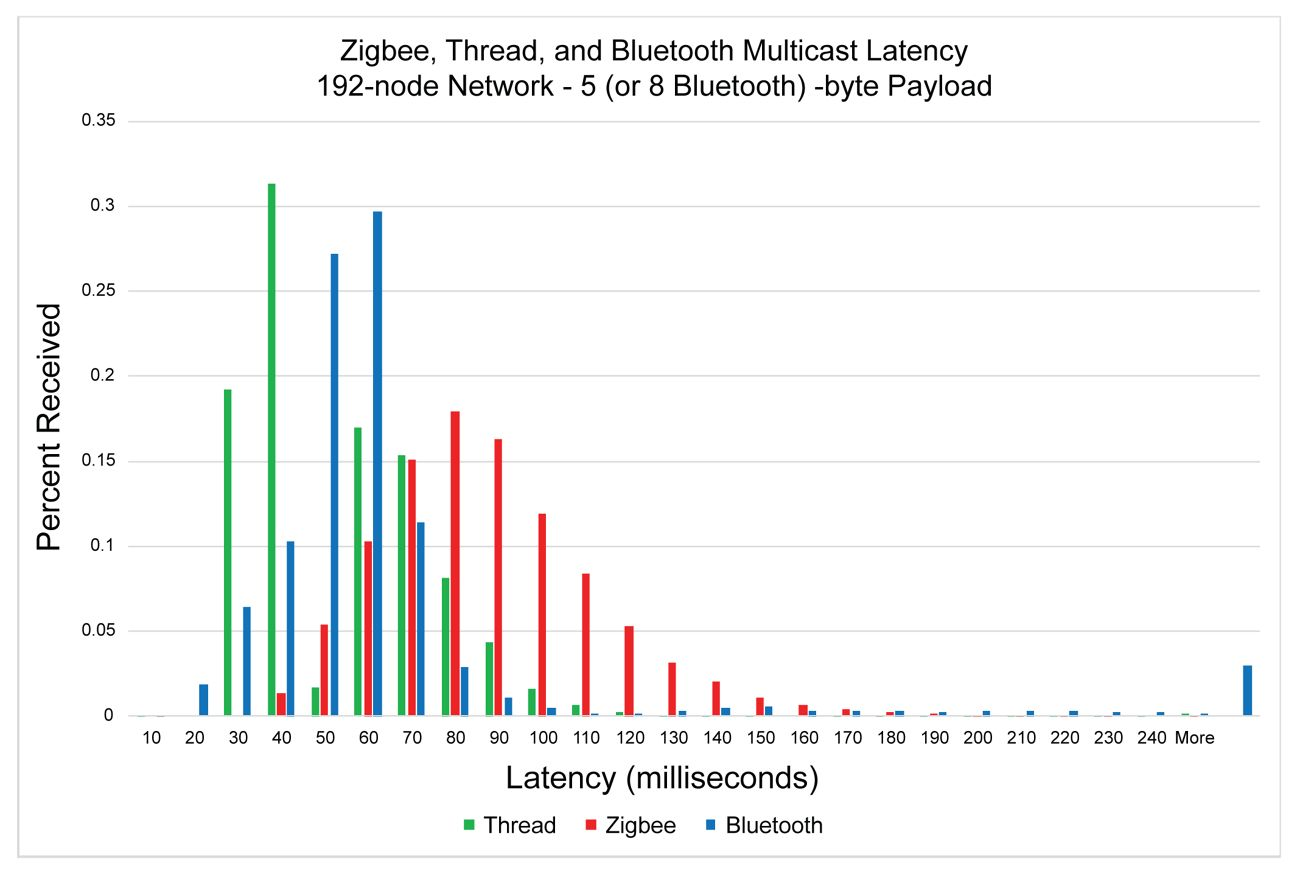
\includegraphics[width=\textwidth]{img/mesh-large-network-small-payload.png}
    \caption{Latency distribution of mesh networks for small data}
    \label{fig:threadsmallload}
    \cite{threadSilabs}
\end{figure}
\noindent
The second measurement tests a mesh network with 192 devices with small (5-8 bytes) and medium (16-25 bytes) data packets and examines the latency distribution.
\newline
For small data, the latencies are distributed as shown in Figure \ref{fig:threadsmallload}. From this, the convention can be drawn that on average, data arrived in 50\,\si{\milli s} for Thread, which performs the best of all mesh networks that were examined. The second best performing is the Bluetooth Mesh, with data arriving in 60\,\si{\milli s} most of the time. However, it is important to note that in 5\% of the measured results, the latency is more than 100\,\si{\milli s}. In the case of Thread, all data arrives in less than 120\,\si{\milli s}. ZigBee performs the worst in this measurement, with an average of 80\,\si{\milli s}, but 190\,\si{\milli s} is the longest delay.

\begin{figure}[!h]
    \centering
    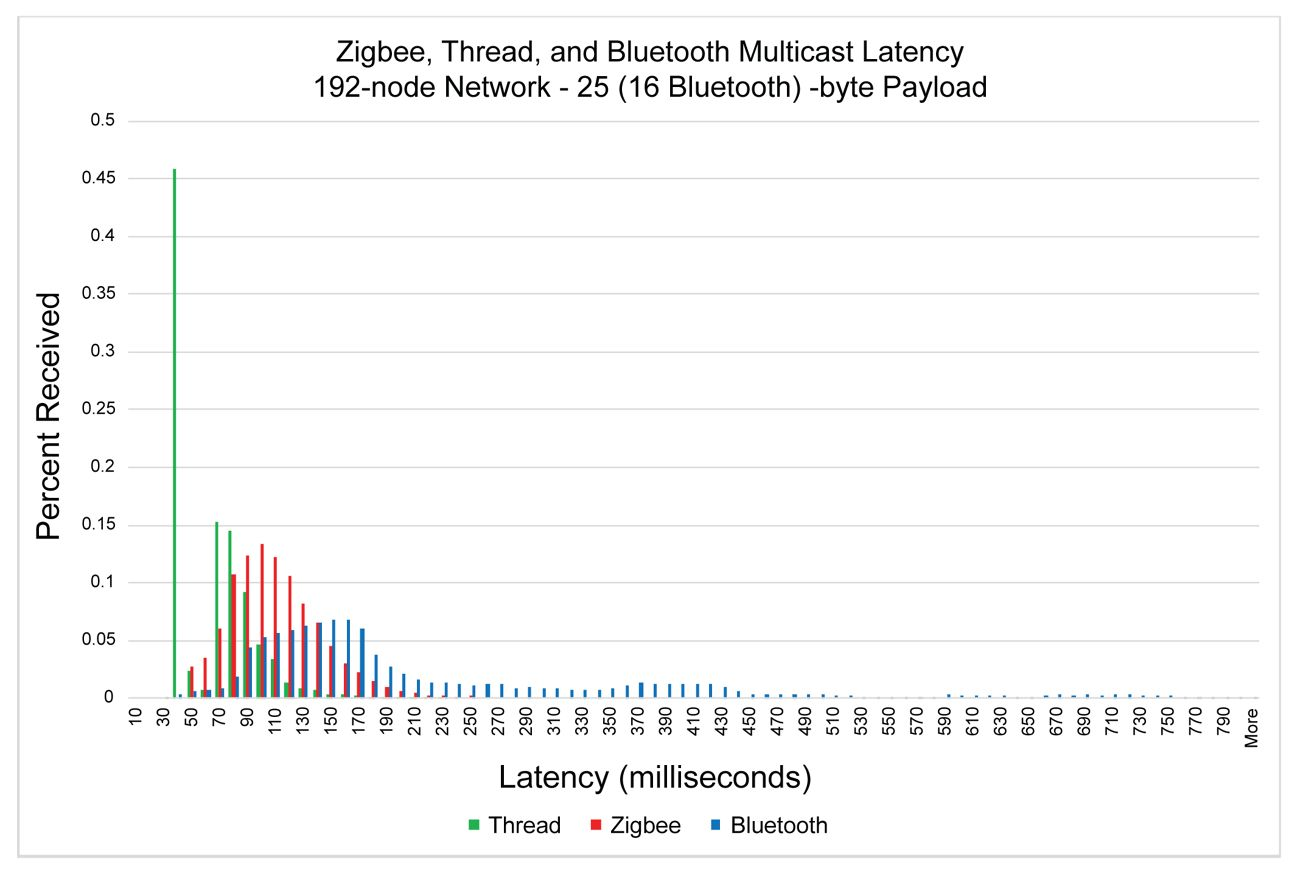
\includegraphics[width=\textwidth]{img/mesh-large-network-moderate-payload.png}
    \caption{Latency distribution of mesh networks for medium data}
    \label{fig:threadmoderateload}
    \cite{threadSilabs}
\end{figure}
\noindent
For larger data, the measurement results are shown in Figure \ref{fig:threadmoderateload}. For Thread, most data reaches the endpoint in 50\,\si{\milli s} on average. This is followed by ZigBee, where this number is 100\,\si{\milli s}. Bluetooth Mesh performed the worst, with data arriving in 150\,\si{\milli s}. It is also important to look at the extreme values. For Thread, the maximum latency is 170\,\si{\milli s}, for ZigBee it is 250\,\si{\milli s} and for Bluetooth Mesh it is up to 750\,\si{\milli s}. From an automation point of view, 750\,\si{\milli s} is not a large delay for a light or a door opener, but for a user to switch these devices using their mobile phone, this would be a very large, noticeable delay.
\newline
The final conclusion from these measurements is that, the Thread performs best in data latency. Thus, for places where data transfer rates of 250\,\si{\kilo bit/s} are sufficient, Thread is the best choice, as it can provide a stable connection with low latency and low power consumption.


\subsection{Thread network}
\begin{figure}[!htb]
    \centering
    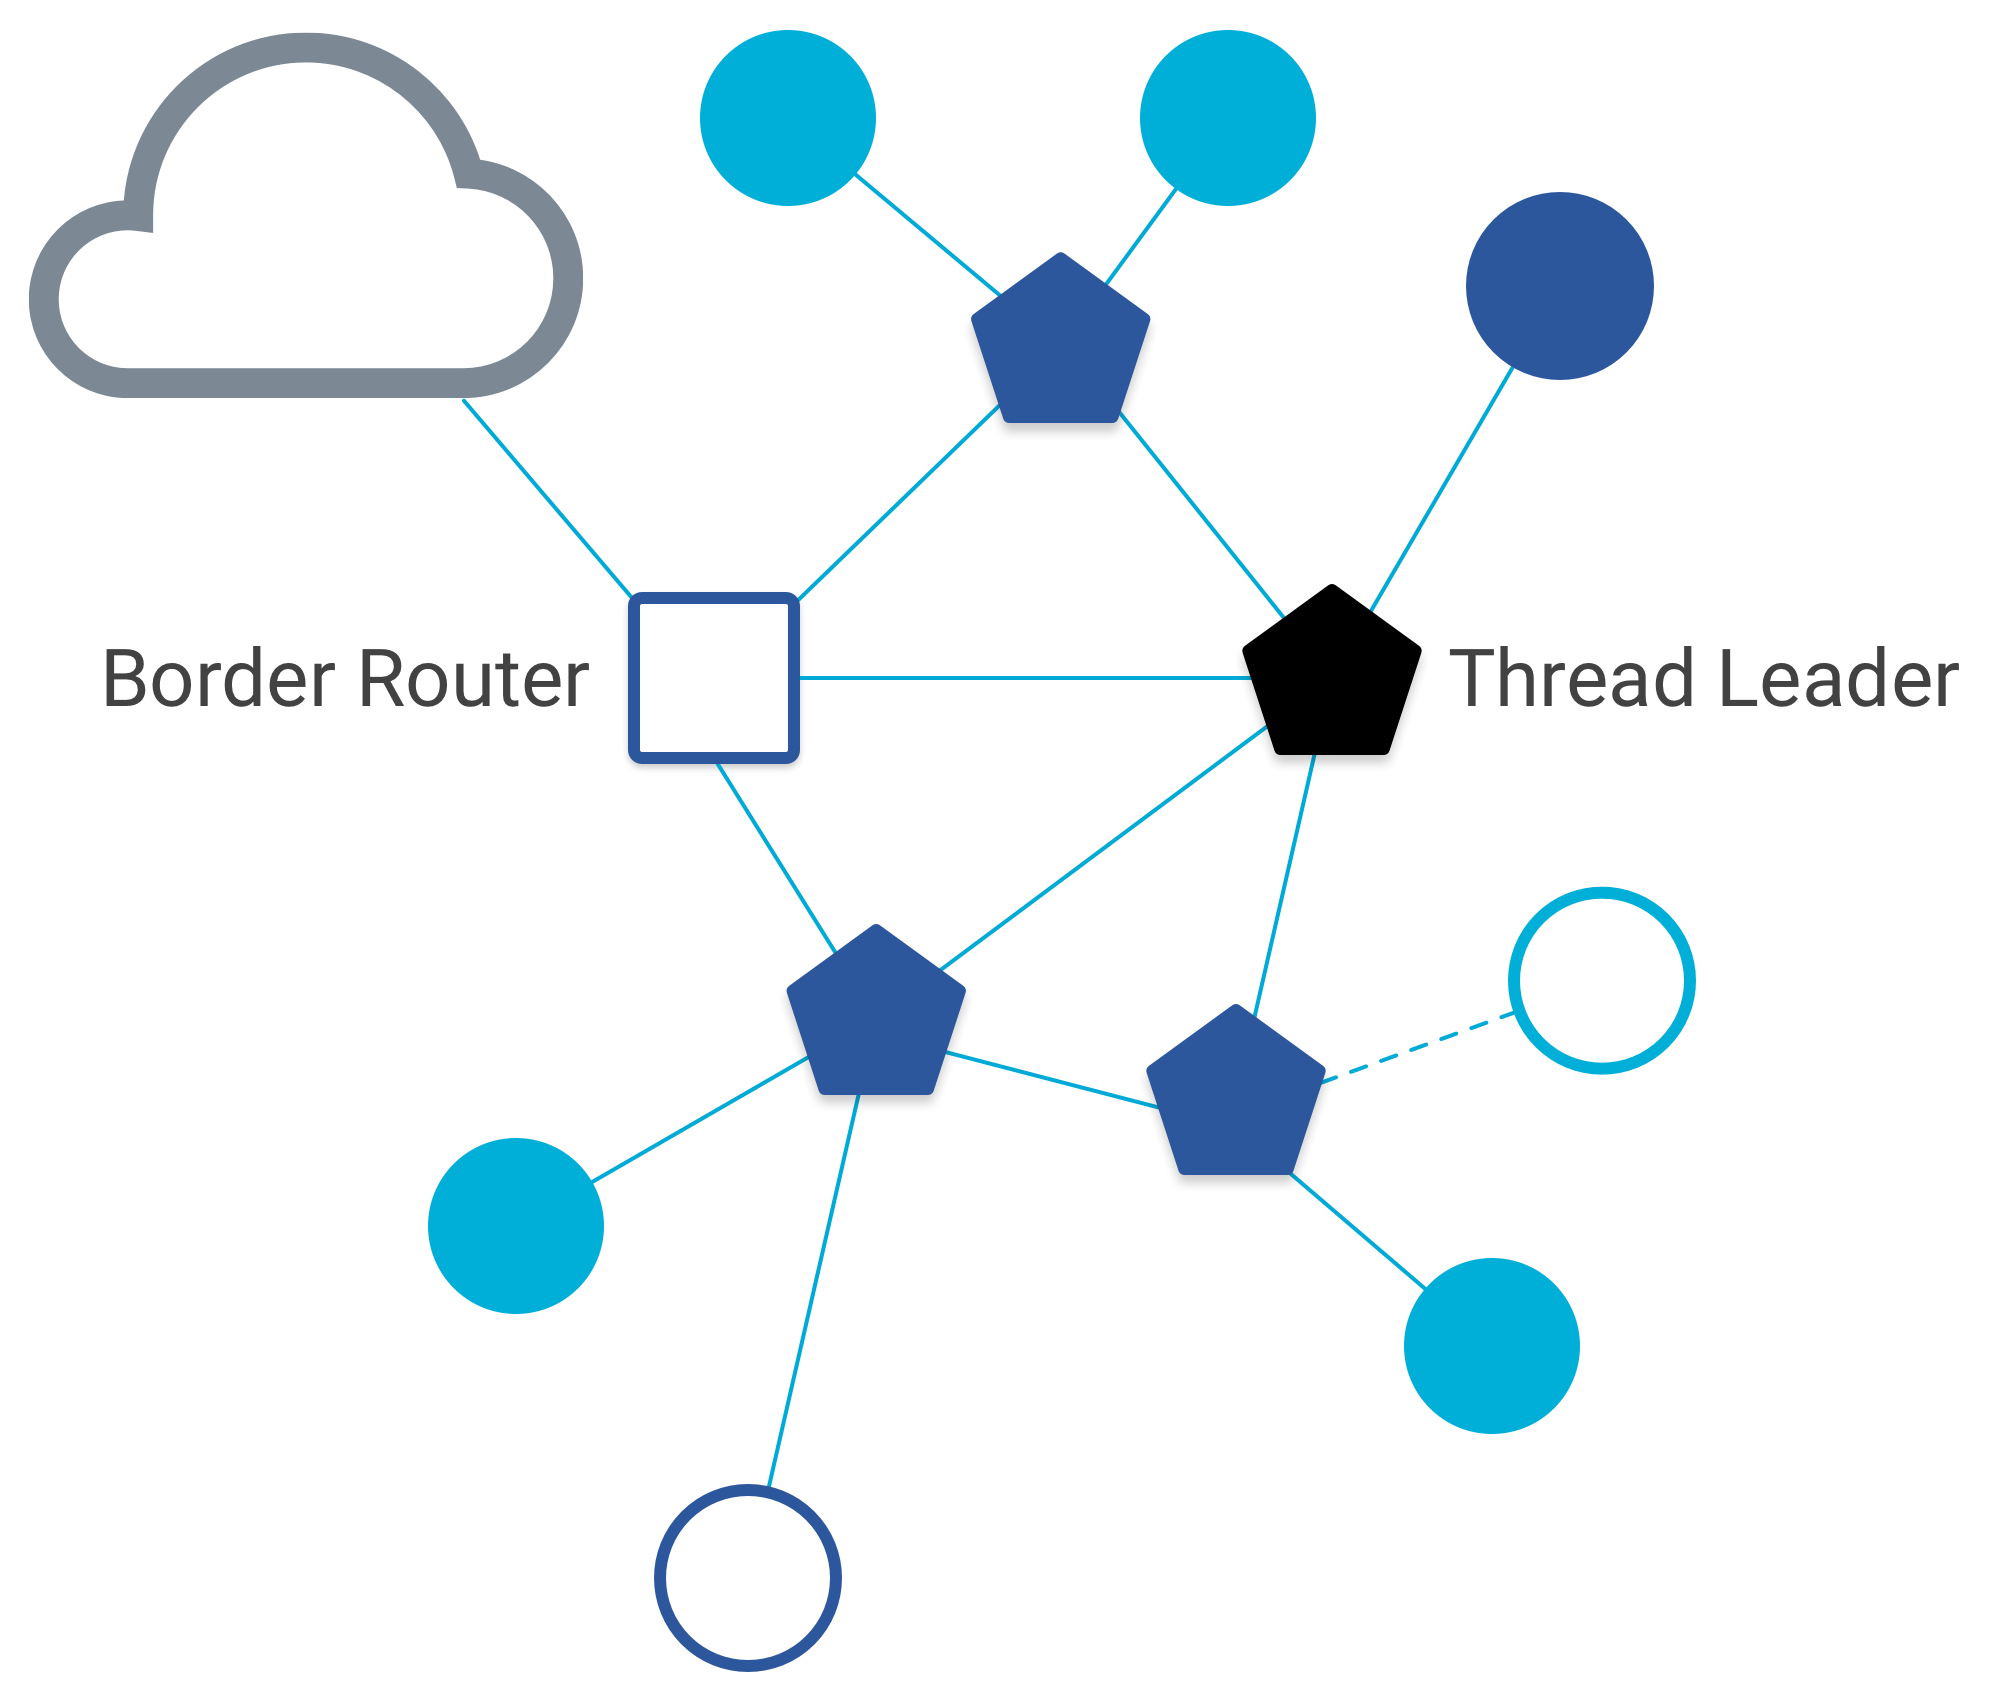
\includegraphics[scale=0.14]{img/ot-primer-leader_2x.png}
    \caption{Thread network topology}
    \label{fig:thread_network}
    \cite{thread_network}
\end{figure}
\noindent
Figure \ref{fig:thread_network} shows a typical Thread network topology. Each blue pentagon represents a Router. These devices can be connected to by so-called End Devices. It is important to note that two types of devices are defined within the Thread protocol. One is the \textit{Full Thread Device}, abbreviated \textbf{FTD} and the other is the \textit{Minimal Thread Device}, abbreviated \textbf{MTD}. The former is recommended in an environment where the continuous power supply for the device is provided (e.g. 230\,\si{\volt} power supply). Because only this kind of devices can form the backbone of the network (see pentagons). Since these devices are responsible for maintaining and managing the IP address topology and sending data within the Thread network. The RF transceiver of Thread FTD devices is always on and subscribes to the multicast address (a pre-booked IP address that can be used to reach a group of devices) of each router and must therefore handle multicast requests. This results in increased power consumption, with a current consumption of 12-15\,\si{\milli\ampere} at a supply voltage of 5\,\si{\volt}, which shows that this devices would not meet the requirement of being able to operate for years from a single coin-cell battery. This problem is solved by Thread MTD devices. As these devices can only communicate with the router or also known as the Parent device. These devices are then called Child and only need to serve requests from the Router, further reducing power consumption. This document refers to Figure \ref{fig:thread_network} in parentheses at the end of the following lists for clarity.
\noindent
FTD devices can perform three functions, which can be\cite{OpenThreadNodeType}
\begin{itemize}
    \item Router (dark blue filled pentagon) --- device that performs network functions,
    \item Router Eligible End Device - REED --- able to designate itself as a router (dark blue filled circle),
    \item Full End Device - FED --- not able to designate itself as a router (dark blue unfilled circle).
\end{itemize}
\clearpage
\noindent
Furthermore, there are three specific states of an FTD device, which are 
\begin{itemize}
    \item Thread Leader (black filled pentagon) --- router management device,
    \item Border Router (dark blue square) --- gateway/transmitter between Thread and other network,
    \item Commissioner (not shown) --- device that performs connectivity.
\end{itemize}
MTD devices can be equipped with two special conditions
\begin{itemize}
    \item Minimal End Device - MED --- in constant contact with the parent,
    \item Sleepy End Device - SED --- is usually in a sleeping state and needs to interrogate the parent upon waking.
\end{itemize}
In this section I introduced the types of devices in a Thread network, but it is important to highlight some of the more important roles.


\subsection{Detailed description of Thread network roles}
\subsubsection{Role of Router}
As I mentioned in the previous section in the case of a Router, the transceiver is always on, as these devices are always FTDs. It's main tasks are to forward packets between devices and to communicate with End Devices. It's special role can be that only these units can connect a new device to the Thread network. I'm going to discuss this process later for the Commissioner.

\subsubsection{Role of End Device/Child}
In this role there is a difference in the operation between MTD and FTD devices, but they have one thing in common. These devices are only connected to one Router and can only communicate with it. They cannot send data directly to other units.
For MTD devices, the transceiver can be optionally disabled to reduce power consumption.

\subsubsection{Role of Thread Leader}
These devices are unique to a Thread network and have the specific task of controlling Router devices and managing configuration information for the entire network. These devices (Routers) dynamically assign themselves to this task to reduce the chance of network failure. The possibility of reassigning device roles usually occurs every 130 seconds. 

\subsubsection{Role of Border Router}
These devices are able to establish a connection between a Thread network and an external network, for example they can act as a gateway. An external network can be an Ethernet network, such as the one I implemented in my bachelor's thesis. Any device can act as a Border Router, there is no restriction, but it is worth choosing an FTD device for this purpose, because it allows continuous communication with the outside world. 

\subsubsection{Role of Commissioner}
As I mentioned in the role of routers, this is an extra task that only Routers can handle. This task is nothing more than connecting new devices to the network. This commissioning is done with an identifier stored in a unique chip called eui64. If this unique identifier is recognised by the Commissioner, the device to be connected can connect to the network using the Joiner password. The Thread Group, Google's developer of OpenThread, also offers various solutions to the connectivity problem, that are as ready-made solutions for developers and users alike.

\subsection{IPv6 addressing within a Thread network}
\begin{figure}
    \centering
    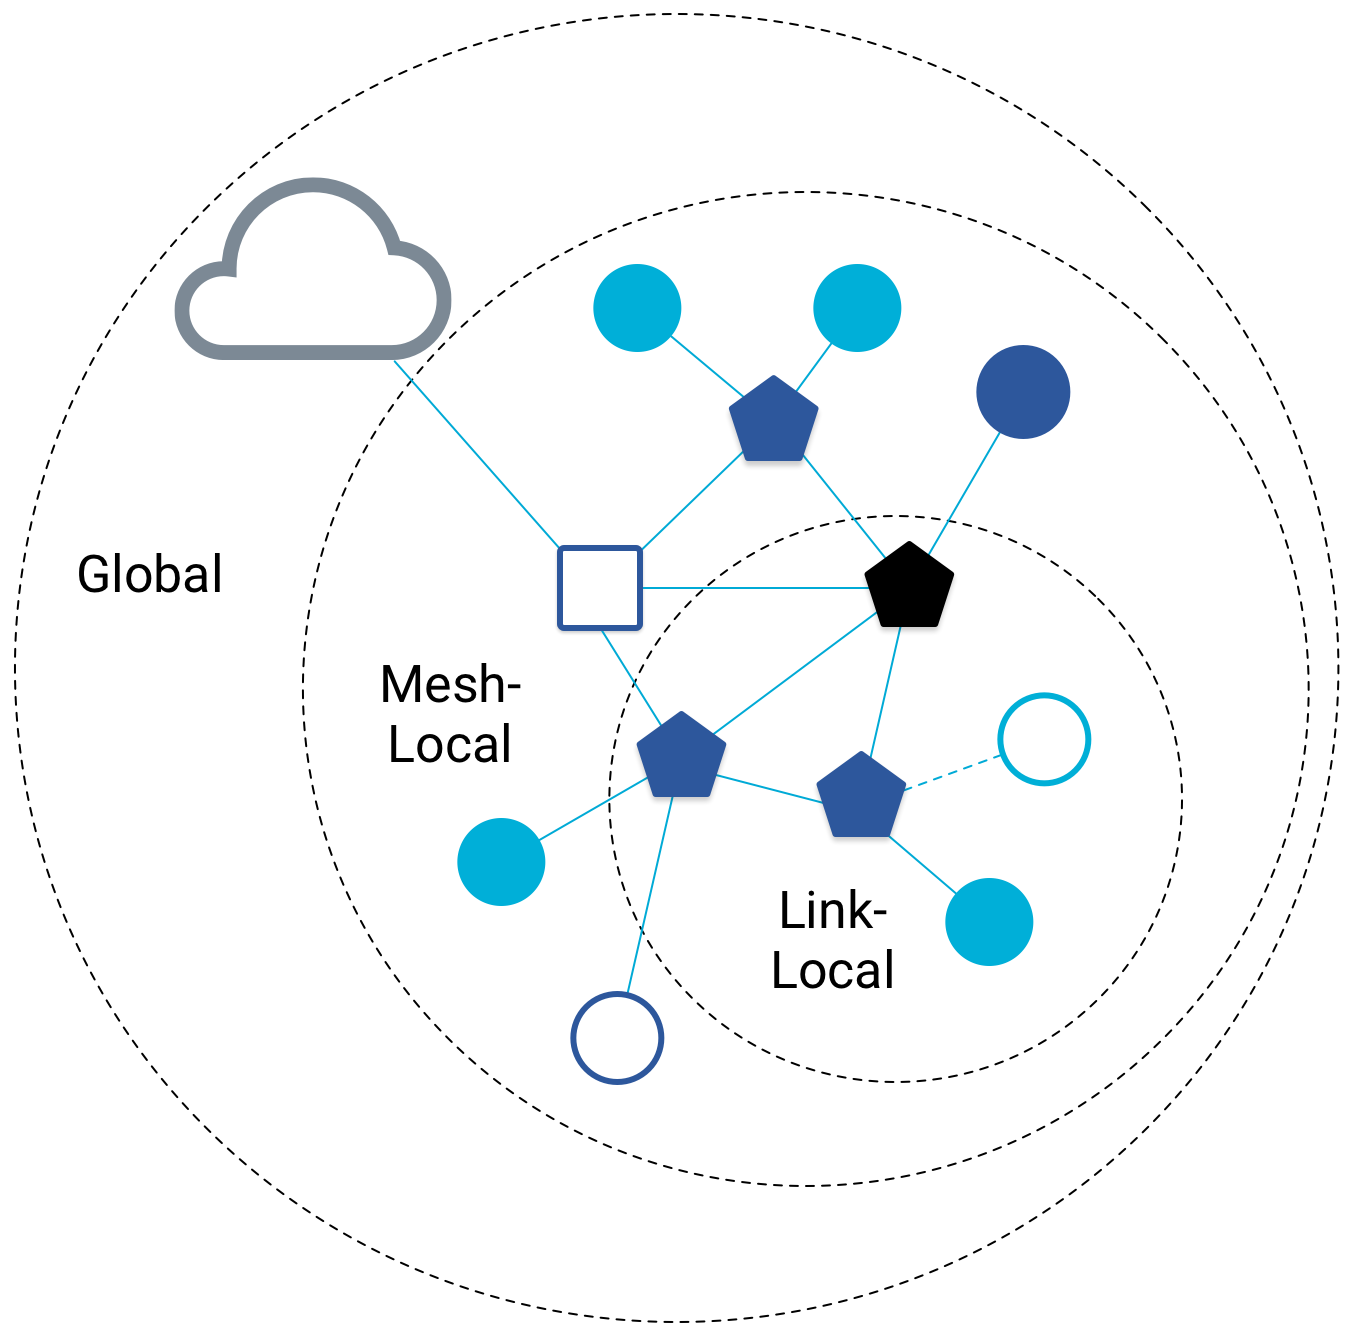
\includegraphics[scale=0.16]{img/ot-primer-scopes.png}
    \caption{Thread network allocation}
    \label{fig:thread_scope}
    \cite{thread_scope}
\end{figure}

Figure \ref{fig:thread_scope} shows that a network can be divided into three main parts.\cite{ThreadIPv6}
\begin{itemize}
    \item Link-Local - prefix: fe80::/16 --- This network contains the devices that are adjacent to each other, i.e. they are reachable by a radio transmission. Generally used to map neighbouring devices.
    \item Mesh-Local - prefix: fd00::/8 --- This network contains all devices that are connected to the given Thread network.
    \item Global - prefix: 2000::/3 --- Devices in this network are accessible from outside the Thread network.
\end{itemize}

\subsubsection{Mesh-Local address role}
These addresses have a more complex function and can be used to send data within the network. They can be divided into two groups, which are
\begin{itemize}
    \item Routing Locator,
    \item Mesh-Local EID.
\end{itemize}
The address \textit{Routing Locator}, also known as \textbf{RLOC} is used to infer the location of a device in the network and also the role of that device. With the \textit{Mesh-Local Endpoint Identifiers} (short \textbf{EID}) any device can be reached within the same Thread network. The Mesh-Local address is the most important one in my bachelor's thesis, as it is the address that allows us to reach all devices connected to the network from the Border Router device such as send and receive information. I am going to show an example of how to manage own devices and send data to them from a website later on.


\subsection{The CoAP protocol}
The \textit{Constrained Application Protocol} or \textbf{CoAP} is an information transfer server-client connection protocol specifically designed for IoT devices. It is very similar to the HTTP protocol known from the Internet, but since IoT devices are often low-powered, HTTP's implementation would consume a lot of resources and thus increase the cost of producing the devices. CoAP is a solution to this problem, taking up to 10\,\si{\kilo B} of RAM and 100\,\si{\kilo B} of code memory from the device's resources.\cite{coap_ram}
\begin{figure}
    \centering
    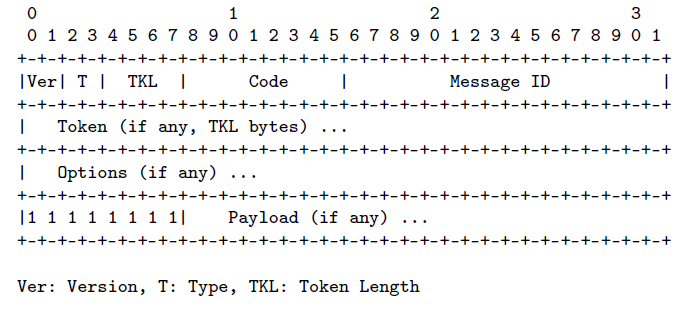
\includegraphics[width=\textwidth]{img/coapframe.png}
    \caption{Format of a CoAP message}
    \label{fig:coapmessage}
    \cite{coapcheat}
\end{figure}
Figure \ref{fig:coapmessage} shows how a CoAP message is constructed. The first two bytes represent the version number and the next two bytes contain the message type, which can take four different values.

\begin{itemize}
    \item Request type messages (Request)
        \begin{itemize}
            \item 0 - \textbf{CON}firmable --- This message type is waiting for an ACK response.
            \item 1 - \textbf{NON}-confirmable --- No response is expected from this message type.
        \end{itemize}
    \item Response type messages (Response)
        \begin{itemize}
            \item 2 - \textbf{ACK}nowledgement --- Confirming response message (see confirmable).
            \item 3 - \textbf{R}e\textbf{S}e\textbf{T} --- This message indicates that the message has been received but the processing result is unsuccessful.
        \end{itemize}
\end{itemize}
\noindent
On Figure \ref{fig:coapmessage}, the \textit{Token Length} (short \textbf{TKL}) indicates the length of the optional symbol (Token) part in four bits. Then the following one-byte code part (\textit{Code}) can be divided into two parts, a three-bit type (\textit{Class}) and a four-bit code (\textit{Code}). Suppose that the client sends a GET request to the server. The request methods are of class 0 and specifically the GET method is denoted by the value 1. If we want to denote this on paper, we separate the class and the code with a dot, so the GET request is denoted by 0.01. The \textit{Message ID} (short \textbf{MID}) is a 16-bit number used to avoid possible message duplications. The Token part is an automatic client-generated number of length defined in the TKL, which must be returned to the server without modification. The purpose of the Token is to allow the client to pair the response to the request. The settings section contains the settings related to the message, such as the address (Uri-Path) used by the intended devices to make the queries or the type of the message content, which can be either a UTF-8 encoded text or even a JSON format. In that case, when the device is needed to save memory, the application should be implemented with CBOR, which has a similar structure to JSON, but the data is encoded in binary format. So the result is more compact, smaller, but not human-readable. After that, a part of one byte and 0xFF separates the actual data from the parts we have seen so far. The detailed specification of the CoAP protocol is available at \href{https://datatracker.ietf.org/doc/html/rfc7252}{datatracker.ietf.org}\cite{datatracker}

\subsection{Summary of Thread}
In this section, I compared three different mesh networking protocol, namely Thread, ZigBee and Bluetooth Mesh and one other protocol, which can operate as a mesh network, Wi-Fi. The basis of this comparison was the power consumption, data speed and the measured latency. On the other hand, the device roles in the Thread network were presented together with the full topology and the CoAP protocol used by OpenThread.